\section{Durchführung}
\label{sec:Durchführung}

% Was wurde gemessen bzw. welche Größen wurden variiert?

Zunächst wird der Versuch nach \autoref{fig:leucht} aufgebaut.

\begin{figure}
    \centering
    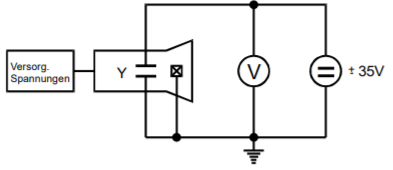
\includegraphics[width=0.5\textwidth]{images/bild3.png}
    \caption{Skizze des Versuchaufbaus für die Leuchtfleckverschiebung.\cite{V501}}
    \label{fig:leucht}
\end{figure}

Im Folgenden wird der Zusammenhang zwischen Leuchtfleckverschiebung und der Ablenkspannung $U_\text{D}$ untersucht.
Auf dem Koordinatennetz befinden sich neun äquidistante Linien.
Die Ablenkspannung ist so einzustellen, dass der Elektronenstrahl nach einander auf alle Linien gerichtet ist.
Für diese Stellen ist jeweils die Spannung abzulesen.
Dieser Vorgang wird für fünf verschiedene Beschleunigungsspannungen $U_\text{B}$ wiederholt, dabei sollte diese Spannung zwischen $\SI{180}{\volt}$ und $\SI{500}{\volt}$ liegen.

Für den zweiten Teil des Versuches wird das Experiment nach \autoref{fig:oszillo} umgebaut.

\begin{figure}
    \centering
    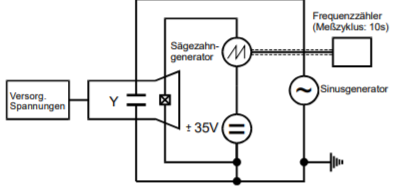
\includegraphics[width=0.6\textwidth]{images/bild4.png}
    \caption{Skizze des Versuchaufbaus für einen Kathodenstrahl-Oszillographen.\cite{V501}}
    \label{fig:oszillo}
\end{figure}

Damit wurde nun ein Kathodenstrahl-Oszillograph gebaut, dieser kann den zeitlichen Verlauf einer einlaufenden Wechselspannung anzeigen.
Am Sägezahngenerator können nun verschiedene Frequenzen $\nu _\text{Sä}$ eingestellt werden.
Die Frequenz einer eingehenden Sinusspannung ist zu notieren.
Dann wird $\nu _\text{Sä}$ so variiert, dass die Frequenz über den Faktor  

\begin{equation}
    n = \frac{1}{2}, \, 1, \, 2, \, 3
\end{equation}

die Frequenz der Sinusspannung ergibt. 
Die Sägezahnfrequenzen werden notiert.